\documentclass[ucs, notheorems, handout]{beamer}

\usetheme[numbers,totalnumbers, nologo]{Statmod}
\usefonttheme[onlymath]{serif}
\setbeamertemplate{navigation symbols}{}

\mode<handout> {
	\usepackage{pgfpages}
	%\setbeameroption{show notes}
	%\pgfpagesuselayout{2 on 1}[a4paper, border shrink=5mm]
	\setbeamercolor{note page}{bg=white}
	\setbeamercolor{note title}{bg=gray!10}
	\setbeamercolor{note date}{fg=gray!10}
}

\usepackage[utf8x]{inputenc}
\usepackage[T2A]{fontenc}
\usepackage[russian]{babel}
\usepackage{tikz}
\usepackage{ragged2e}

\usepackage{multirow}

%\usepackage{multirow}
%\usepackage[table,xcdraw]{xcolor}

\newtheorem{theorem}{Теорема}
\newtheorem*{definition}{Определение}
\newtheorem{lemma}{Лемма}
\usepackage{amsmath}
\usepackage{amsthm}
\usepackage{bm}
\usepackage{bbold}

\usepackage{pgfplots}
\pgfplotsset{compat=1.9}

\usepackage{graphicx}
%\usepackage[usenames]{color}
%\usepackage{colortbl}

%\newtheorem{theorem}{Теорерма}
\newtheorem{corollary}[theorem]{Следствие}
%\newtheorem{lemma}[theorem]{Лемма}
\newtheorem{observation}[theorem]{Observation}
\newtheorem{proposition}[theorem]{Предложение (Swanson)}
\newtheorem{proposition2}[theorem]{Предложение}
%\newtheorem{definition}[theorem]{Определение}
\newtheorem{claim}[theorem]{Утверждение}
\newtheorem{fact}[theorem]{Факт}
\newtheorem{assumption}[theorem]{Предположение}
\newtheorem{alg}{Алгоритм}
\newtheorem{zam}{Замечание}

\newtheorem{example}{Пример}[section]

\newenvironment{Proof}{\par\noindent{\bf Доказательство.}}{\hfill$\scriptstyle\blacksquare$}
\newenvironment{ex}{\par\noindent{\bf Пример.}}{}
\newenvironment{pr1}{\par\noindent{\bf Дано:}}{}
\newenvironment{pr2}{\par\noindent{\bf Шаги:}}{}
\newenvironment{pr3}{\par\noindent{\bf Результат:}}{}

\DeclareMathOperator{\tr}{tr}
\DeclareMathOperator{\F}{\mathsf{F}}

\title[Замена непрерывного распределения]{Замена непрерывного распределения на дискретное для применения на практике}
\author[Нагуманова~К. И.]{ Нагуманова Карина Ильнуровна, 19Б.04-мм}

\date{\tiny{Санкт-Петербург\\ 2023г.}}
\institute[Санкт-Петербургский Государственный Университет]{%
	\small
	Санкт-Петербургский государственный университет\\
	Математико-механический факультет\\
	Кафедра статистического моделирования\\
	\vspace{0.8cm}
	Научный руководитель: д.ф.-м.н., доцент Голяндина Н.\,Э.\\
	Рецензент: лектор Кардиффского университета Пепелышев А.\,Н.
	%Вычислительная стохастика и статистические модели\\
	\vspace{1cm}}
	
\begin{document}
	
	\begin{frame}
		\titlepage
		\note{Научный руководитель  д.ф.-м.н., доцент Голяндина Н.\,Э.,\\
			кафедра статистического моделирования}
	\end{frame}
	
	\begin{frame}{Введение}
		
		В практических задачах нередко требуется заменить непрерывное распределение на
		дискретное с сохранением математического ожидания и дисперсии. Одним из методов
		нахождения такого распределения для трехточечной аппроксимации нормального распределения является \textcolor{blue}{\hbox{\textbf{метод Свонсона}}}.
		
		\bigskip
		
		Аппроксимируемые случайные величины складывают и умножают.
		
		\bigskip
		
		\textcolor{red}{\textbf{Задача:}} находить аппроксимацию суммы и произведения логнормальных случайных величин по аппроксимациям исходных случайных величин.
		
		\note{В практических задачах нередко требуется заменить непрерывное распределение на
			дискретное с сохранением математического ожидания и дисперсии. Одним из методов
			нахождения такого распределения для трехточечной аппроксимации нормального распределения является метод Свонсона. Однако в ряде областей, например, в нефтяной промышленности, общепринятым распределением, описывающим запасы нефти, является логнормальное распределение. 
			Соответственно, реальной задачей является аппроксимация логнормального распределения. При этом здесь тоже применим метод Свонсона, потому что логнормальное распределение можно свести к нормальному. Ставится задача нахождения аппроксимации суммы и произведения логнормальных случайных величин по аппроксимациям исходных случайных величин.}
	\end{frame}
	
	
	\begin{frame}{Введение}
		\textbf{План работы.}
		\begin{enumerate}
			\medskip
			\item Рассмотреть общий подход к трехточечной аппроксимации,трехточечную аппроксимацию нормального распределения, метод Свонсона и вывод правила 30-40-30.
			\medskip
			\item Рассмотреть трехточечную аппроксимацию логнормального распределения и её  свойства.
			\medskip
			\item Построить алгоритм аппроксимации произведения двух логнормальных распределений.
			\medskip
			\item Построить алгоритм аппроксимации суммы двух логнормальных распределений.
		\end{enumerate}
	
	\note{Имеем следующий план работы. Рассмотреть общий подход к трехточечной аппроксимации, рассмотреть трехточечную аппроксимацию нормального распределения, в целом метод Свонсона и вывод правила 30-40-30, рассмотреть трехточечную аппроксимацию логнормального распределения и её  свойства, построить алгоритм аппроксимации произведения двух логнормальных распределений, построить алгоритм аппроксимации суммы двух логнормальных распределений.}
	\end{frame}
	
	\begin{frame}{Часть 1: Общий подход к трехточечной аппроксимации}
		Пусть $\xi$ "--- непрерывная случайная величина, обозначим  \[m = \mathbf E(\xi), \quad\quad s^{2} = \mathbf D(\xi),\]  $F(x)$ "--- функция распределения,
		$x_{\pi_{1}}$, $x_{\pi_{2}}$, $x_{\pi_{3}}$ "--- квантили $\xi$,
		
		$\tilde{\xi}$ "--- дискретная случайная величина 
		
		\[\tilde{\xi}:\quad\begin{pmatrix} 
			x_{\pi_{1}}&x_{\pi_{2}}&x_{\pi_{3}}\\ 
			p_{1} &  p_{2}  & p_{3}
		\end{pmatrix}\]
		
		\[\tilde{m} = \mathbf E(\tilde{\xi}), \quad\quad \tilde{s}^{2} = \mathbf D(\tilde{\xi}).\]
		\textcolor{red}{\textbf{Задача:}} аппроксимировать распределение случайной величины $\xi$ дискретным распределением $\tilde{\xi}$, то есть найти $p_{1}$, $p_{2}$, $p_{3}$ такие, что 
		\begin{equation*}
			p_{1} + p_{2} + p_{3} = 1, \label{1}
		\end{equation*}
		\begin{equation*}
			\tilde{m} = p_{1}x_{\pi_{1}} + p_{2}x_{\pi_{2}} + p_{3}x_{\pi_{3}} = m, \label{2}
		\end{equation*}
		\begin{equation*}
			\tilde{s}^{2} = p_{1} x_{\pi_{1}}^{2} + p_{2} x_{\pi_{2}}^{2} + p_{3} x_{\pi_{3}}^{2} - m^{2} = s^{2}. \label{3}
		\end{equation*}
		
		\note{Пусть $\xi$ "--- непрерывная случайная величина, вводим основные обозначения для $\xi$, так же вводим дискретную случайную величину, которой будем аппроксимировать $\xi$. Ставится задача аппроксимации распределения $\xi$ дискретным распределением $\tilde{\xi}$, то есть нужно вычислить $p_{1}$, $p_{2}$, $p_{3}$ такие, что верны следующие равенства. }
	\end{frame}
	
	\begin{frame}{Часть 1: Аппроксимация нормального распределения}
		\begin{proposition}\label{pr1}
			Пусть верно 
			\begin{equation*}
				\begin{pmatrix} 
					1&1&1\\ 
					\hat{x}_{\pi_{1}}~~ &  \hat{x}_{\pi_{2}}~~  & \hat{x}_{\pi_{3}} \\ 
					\hat{x}_{\pi_{1}}^{2}~~&\hat{x}_{\pi_{2}}^{2}~~  &\hat{x}_{\pi_{3}}^{2}
				\end{pmatrix}
				\begin{pmatrix}p_{1}\\p_{2}\\ p_{3}\end{pmatrix}= \begin{pmatrix}1\\0\\1 \end{pmatrix},\label{4}
			\end{equation*}
			где $\hat{x}_{\pi_{i}} = \hat{\F}^{-1}(\pi_{i})$, $\hat{\F}(y)$ "--- функция распределения $\displaystyle{\hat{\xi} = \frac{\xi-m}{s}}$. Тогда $m=\tilde{m}$ и $s^{2} = \tilde{s}^{2}$.
		\end{proposition}
	
	Рассмотрим частный случай $\xi\sim N(\mu, \sigma), \pi = 0.1$, имеем 
	$$\Phi ^{-1}(0.1) = -\Phi ^{-1}(0.9) \approx  -1.28, \qquad \Phi ^{-1}(0.5) = 0, $$
	$$p_{1}\approx 0.305, \qquad p_{2}\approx 0.390, \qquad p_{3}\approx 0.305.$$
	
	Эти вероятности примерно равны 0.3, 0.4, 0.3, поэтому это правило называют \textcolor{blue}{\hbox{\textbf{правилом 30-40-30}}}.
	
	\note{Пусть верна следующая система, тогда $m=\tilde{m}$ и $s^{2} = \tilde{s}^{2}$. Это Предложение дает требуемую аппроксимацию дискретным распределением, если найденные вероятности $p_{i}$ являются неотрицательными. }
		
		%\bigskip
	\end{frame}
	
	\begin{frame}{Часть 2: Связь логнормального с нормальным}
		Пусть $\xi = \ln(\eta)$ и $\xi \sim N(\mu, \sigma)$. Параметры $m = \mathbf E(\eta)$, $s^{2} = \mathbf D(\eta)$ логнормального распределения выражаются как
		\[m = \exp\left( \mu + \dfrac{\sigma^{2}}{2}\right), \quad\quad s^{2} = \exp\left( 2\mu +\sigma^{2}\right)(\exp(\sigma^{2})-1).\]
		Обратная функция распределения $\eta$ имеет вид
		\begin{equation*}
			F_{\eta}^{-1}(p) = \exp(\mu+\sigma\sqrt{2}\mathrm{erf}^{-1}(2p-1)). \label{10}
		\end{equation*}
	\begin{proposition2}
		Параметр $\mu$ выражается как $\mu = \log(x_{\pi_{i}}) - \sigma\Phi ^{-1}(\pi_{i})$
		и результат не зависит от $i$.
		Параметр $\sigma$ выражается через любые два квантиля как
		\begin{equation*}
			\displaystyle{\sigma = \dfrac{\log\left(\dfrac{x_{\pi_{2}}}{x_{\pi_{1}}}\right)}{\Phi ^{-1}(\pi_{2}) - \Phi ^{-1}(\pi_{1})}}, \quad \quad \pi_{1}\neq \pi_{2}. \label{11}
		\end{equation*} 
	\end{proposition2}
		
	\end{frame}
	
	\begin{frame}{Часть 2: Аппроксимация логнормального распределения}
		\begin{pr1}
			квантили $x_{\pi_{1}}, x_{\pi_{2}}, x_{\pi_{3}}$ логнормальной случайной величины $\eta$, $\ln(\eta) \sim N(\mu, \sigma)$.
		\end{pr1}
		
		\bigskip
		
		\begin{enumerate}
			\item Выражаем параметры $\mu$ и $\sigma$ математическое ожидание и дисперсию соответствующего нормального распределения через известные $x_{\pi_{1}}, x_{\pi_{2}}, x_{\pi_{3}}$.
			\medskip
			\item Вычисляем значения математического ожидания $m$ и дисперсии $s^{2}$ случайной величины $\eta$, используя $\mu$ и $\sigma$.
			\medskip
			\item С помощью системы уравнений находим значения весов $p_{1}$, $p_{2}$, $p_{3}$, используя вычисленные $m$ и $s^{2}$.
		\end{enumerate}
		\bigskip
		\begin{pr3}\end{pr3} веса $p_{1}$, $p_{2}$, $p_{3}$ для $x_{\pi_{1}}, x_{\pi_{2}}, x_{\pi_{3}}$ случайной величины $\tilde{\xi}$.
		
		\medskip
		В реальных задачах в нефтяной промышленности используются следующие диапазоны
		параметров: $\mu \leq 12$, $\sigma \leq 1.5$.
		
		\note{Построим алгоритм для нахождения трехточечной симметричной аппроксимации логнормального распределения. Заданы три квантиля $x_{\pi_{1}}, x_{\pi_{2}}, x_{\pi_{3}}$, вычисляем по ним мат. ожидание $m$ и дисперсию $s^{2}$ случайной величины $\eta$. Затем выражаем параметры $\mu$ и $\sigma$ и наконец находим значения весов $p_{1}$, $p_{2}$, $p_{3}$.}
	\end{frame}
	
	\begin{frame}{Часть 2: Условие на параметр $\sigma$}
		Мною было доказано следующее предложение.
		\begin{proposition2}
			Неотрицательные вероятности $p_{1}$, $p_{2}$, $p_{3}$ для аппроксимации логнормальной случайной величины $\eta$ в точках $\pi$-, $0.5$- и $(1-\pi)$- квантилей существуют только при условии \[\exp(\sigma^{2})+\exp(-\sigma^{2})-\exp\left( -\dfrac{\sigma^{2}}{2}\right) 
			(\exp(c\sigma)+\exp(-c\sigma))\leq 0,\] 
			где $c = \Phi^{-1}(\pi)$.
			%(при $\sigma\leq 0.6913$, $\gamma_{3}\leq 2.8278$ примерно).
		\end{proposition2}
		
		\begin{corollary}
			При уменьшении значения $\pi$ диапазон существования дискретной вероятностной аппроксимации увеличивается.
		\end{corollary}
	
	Например, для $\pi = 0.1$ получаем ограничение $\sigma \leq 0.6913$.
	
	\note{Мы рассмотрели способ вычисления весов для квантилей при аппроксимации логнормального распределения. Но найденные веса являются вероятностями не при любом $\sigma$. Выясним, какое должно быть ограничение на этот параметр. В следующем предложении получено условие на $\sigma$ для существования трехточечной симметричной аппроксимации логнормального распределения. При уменьшении значения $\pi$ диапазон значений $\sigma$ увеличивается.}
		
	\end{frame}
	
	\begin{frame}{Часть 2: Точность метода Свонсона для логнормального распределения}
		\textbf{Проблема:} метод Свонсона выведенный для аппроксимации нормального распределения используют для логнормального.
		
		\textbf{Вопрос:} какова точность аппроксимации $m$ и $s^{2}$?
		
		\begin{proposition2}\label{pr5}
			Ошибка аппроксимации мат.ожидания логнормального распределения по методу Свонсона, выведенному для аппроксимации нормального распределения, равна
			\[\dfrac{ m - \widetilde{m} }{m} =  \exp\left( \dfrac{\sigma^{2}}{2}\right)  - \dfrac{1}{2 c^{2}}\times\]\[\times(\exp(c\sigma)-1 +\exp(-c\sigma)) + 1 /\exp\left(\dfrac{\sigma^{2}}{2}\right),\]
			где $c = \Phi^{-1}(\pi)$, и не зависит от параметра $\mu$.
		\end{proposition2}
	
	\note{Предлагаемые методы аппроксимации трехточечным дискретным распределением логнормального распределения не работают при $\sigma \leq 0.6913$. На практике часто используют метод Свонсона выведенный для аппроксимации нормального распределения. Мною доказано это предложение. Ошибка аппроксимации мат. ожидания выражается следующим образом и не зависит от параметра $\mu$. }
	\end{frame}
	
	\begin{frame}{Часть 2: Точность метода Свонсона для логнормального распределения}
		\begin{proposition2}\label{pr6}
			Ошибка аппроксимации дисперсии логнормального распределения по методу Свонсона, выведенному для аппроксимации нормального распределения, равна
			\[\dfrac{ s^{2} - \widetilde{s}^{2} }{s^{2}} = \exp(\sigma^{2})(\exp(\sigma^{2}-1)) -\]\[- \dfrac{1}{2c^{2}}\exp(-2c\sigma)- \left( 1- \dfrac{1}{c^{2}}\right) \exp(2c\sigma)+\]\[+ \left( \dfrac{1}{2c^{2}}(\exp(c\sigma)-1+\exp(-c\sigma)) + 1\right) ^{2} /\exp(\sigma^{2})(\exp(\sigma^{2}-1)),\]
			где $c = \Phi^{-1}(\pi)$, и не зависит от параметра $\mu$.
			
			%\mid
			
		\end{proposition2}
	
	\note{Ошибка аппроксимации дисперсии выражается следующим образом и тоже не зависит от параметра $\mu$.}
	\end{frame}
	
	\begin{frame}{Часть 2: Точность метода Свонсона для логнормального распределения}
		
		\begin{figure}[h]
			\begin{center}
				\begin{minipage}[h]{0.9\linewidth}
					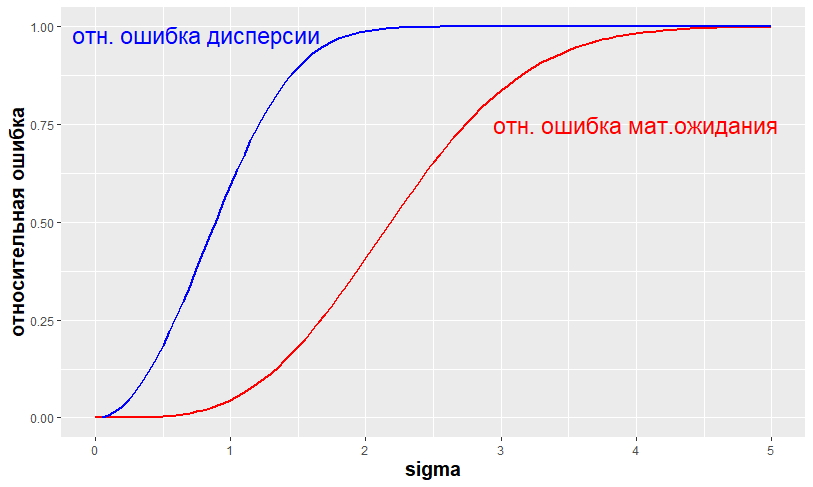
\includegraphics[width=1\linewidth]{img/gr2oh_new2.png}
					\caption{Относительная ошибка аппроксимации математического ожидания и дисперсии} %% подпись к рисунку
					\label{ris:image2} %% метка рисунка для ссылки на него
				\end{minipage}
				
			\end{center}
		\end{figure}
	
	\note{Теперь посмотрим на график зависимости ошибок аппроксимации мат.ожидания и дисперсии от параметра $\sigma$. Видим, что при $\sigma\leq1.5$ ошибка аппроксимации мат.ожидания меньше $12\%$, а ошибка аппроксимации дисперсии может достигать $80\%$. Для интересующих нас значений $\sigma\geq 0.69$ ошибка мат. ожидания может быть как маленькой, так и очень большой. Ошибка дисперсии при этом точно больше $25\%$. }
		
		%Видим, что при $\sigma\leq1.5$ ошибка аппроксимации мат.ожидания меньше $12\%$. 
		%Видим, что при $\sigma\leq1.5$ ошибка аппроксимации дисперсии может достигать $80\%$. 
		
	\end{frame}
	
	
	\begin{frame}{Часть 3: Произведение двух логнормальных распределений}
		
		\begin{proposition}
			Зная квантили $x_{\pi}$, $x_{0.5}$, $x_{1-\pi}$ случайной величины $\xi_{1}$ и квантили $y_{\pi}$, $y_{0.5}$, $y_{1-\pi}$ случайной величины $\xi_{2}$ можно найти квантили $z_{\pi}$, $z_{0.5}$, $z_{1-\pi}$ случайной величины $\xi_{1}\xi_{2}$, как
			
			\begin{equation*}
				z_{\pi}=\exp(b\Phi^{-1}(\pi)+a),
			\end{equation*}
			\begin{equation*}
				z_{0.5}=x_{0.5}y_{0.5},
			\end{equation*}
			\begin{equation*}
				z_{1-\pi}=\exp(b\Phi^{-1}(1-\pi)+a),
			\end{equation*}
			
			где $a$ и $b$ такие, что прямая $y=\dfrac{x-a}{b}$, проходит через точки $(\ln(x_{\pi}y_{\pi}), t)$ и $(\ln(x_{0.5}y_{0.5}),0)$ при
			\begin{equation*}
				t = \frac{\Phi^{-1}(\pi)((\ln(x_{0.5})+\ln(y_{0.5}))-(\ln(x_{\pi})+\ln(y_{\pi})))}{\sqrt{(\ln(x_{0.5})-\ln(x_{\pi}))^{2}+(\ln(y_{0.5})-\ln(y_{\pi}))^{2}}}. 
			\end{equation*}
		\end{proposition}
	
	\note{Следующее предложение было мною подробно доказано, но сама идея доказательства взята из статьи. Зная квантили $x_{\pi}$, $x_{0.5}$, $x_{1-\pi}$ случайной величины $\xi_{1}$ и квантили $y_{\pi}$, $y_{0.5}$, $y_{1-\pi}$ случайной величины $\xi_{2}$ можно найти квантили $z_{\pi}$, $z_{0.5}$, $z_{1-\pi}$ случайной величины $\xi_{1}\xi_{2}$.}
	
	\end{frame}
	
	
	\begin{frame}{Часть 4: Сумма двух логнормальных распределений }
		
		Рассмотрим сумму двух логнормальных случайных величин
		\begin{equation*}
			\ln(\xi_{1}) \sim N(\mu_{1}, \sigma _{1}^{2}),
		\end{equation*}
		\begin{equation*}
			\ln(\xi_{2}) \sim N(\mu_{2}, \sigma _{2}^{2}),
		\end{equation*}
		\begin{equation*}
			\xi = \xi_{1}+\xi_{2},
		\end{equation*}
		где $\xi_{1}$ и $\xi_{2}$ заданы своими квантилями.
		\bigskip
		
		Поставим задачу аппроксимации суммы логнормальным распределением $\ln(\eta)\sim N(\mu, \sigma)$, так как нужно рассматривать сумму не обязательно двух, а произвольного числа случайных величин. 
		
		\bigskip
		
		\textbf{Задача:} найти квантили $z_{\pi}$, $z_{0.5}$, $z_{1-\pi}$ случайной величины $\eta$.
		
		\note{Рассмотрим сумму двух логнормальных случайных величин,которые заданы наборами своих квантилей. Поставим задачу аппроксимации суммы логнормальным распределением $\ln(\eta)\sim N(\mu, \sigma)$, так как нужно рассматривать сумму не обязательно двух, а произвольного числа случайных величин. По известным квантилям уже знаем, как вычислить вероятности $p_{1}$, $p_{2}$, $p_{3}$ такие, что $m = \tilde{m}$  и $s^{2} = \tilde{s}^{2}$.}
		
		
	\end{frame}
	
	\begin{frame}{Часть 4: Сумма двух логнормальных распределений}
		
		\begin{pr1}
			Квантили $x_{\pi}$, $x_{0.5}$, $x_{1-\pi}$ "--- квантили $\xi_{1}$, $y_{\pi}$, $y_{0.5}$, $y_{1-\pi}$ "--- квантили $\xi_{2}$.
		\end{pr1}
		\begin{enumerate}
			\item $x_{\pi}$, $x_{0.5}$, $x_{1-\pi}$ $\rightarrow$  $\mu_{1}$, $\sigma_{1}$
			\item $y_{\pi}$, $y_{0.5}$, $y_{1-\pi}$ $\rightarrow$ $\mu_{2}$, $\sigma_{2}$
			\item $\mu_{i}$, $\sigma_{i}$ $\rightarrow$ $m_{i}$, $s_{i}^{2}$
			\item $m = m_{1}+m_{2}$
			\item $s^{2}=s_{1}^{2} + s_{2}^{2}$
			\item $m$, $s^{2}$ $\rightarrow$ $\mu$, $\sigma$
			\item $\mu$, $\sigma$ $\rightarrow$ $z_{\pi}$, $z_{0.5}$, $z_{1-\pi}$
			\item $z_{\pi}$, $z_{0.5}$, $z_{1-\pi}$ $\rightarrow$ $p_{1}$, $p_{2}$, $p_{3}$
			
		\end{enumerate}
		\begin{pr3}\end{pr3} вероятности $p_{1}$, $p_{2}$, $p_{3}$ для квантилей $z_{\pi_{1}}, z_{\pi_{2}}, z_{\pi_{3}}$ случайной величины $\xi_{1} + \xi_{2}$.
		
		\note{Получен следующий алгоритм аппроксимации суммы двух логнормальных распределений. По набору квантилей $\xi_{1}$ находим параметры $\mu_{1}$, $\sigma_{1}$ соответствующего нормального распределения. По набору квантилей $\xi_{2}$ находим параметры $\mu_{2}$, $\sigma_{2}$ соответствующего нормального распределения. Потом находим мат. ожидания и дисперсии $\xi_{1}$ и $\xi_{2}$. Затем вычисляем мат.ожидание и дисперсию $\xi_{1}+\xi_{2}$. Через них находим параметры нормального распределения и затем находим значения квантилей через $\mu$ и $\sigma$.}
		
	\end{frame}
	
	
	\begin{frame}{Часть 4: Точность аппроксимации }
		
		Oшибки аппроксимации квантилей $q_{\pi}$, $q_{0.5}$, $q_{1-\pi}$ случайной величины $\xi$ равны
		\[\dfrac{\left| q_{\pi} - z_{\pi}\right|}{q_{\pi}}, \quad\quad \dfrac{\left| q_{0.5} - z_{0.5}\right|}{q_{0.5}}, \quad\quad \dfrac{\left| q_{1-\pi} - z_{1-\pi}\right|}{q_{1-\pi}},\] где
		\[z_{100p} = F_{\eta}^{-1}(p) = \exp(\mu+\sigma\sqrt{2}\mathrm{erf}^{-1}(2p-1)).\]
		Значение квантилей $q_{i}$ выражаются как $q_{100p} = F_{\xi}^{-1}(p)$, где
		\[F_{\xi}(x) = \int_{0}^{x}\left( \dfrac{1}{2}+\dfrac{1}{2} \mathrm{erf}\left( \dfrac{\ln(x-y)-\mu_{1}}{\sigma_{1}\sqrt{2}}\right) \right)\times\]
		\[\times \left( \dfrac{1}{\sqrt{2\pi}y\sigma_{2}}\exp\left( -\left( \dfrac{\ln(y)-\mu_{2}}{\sqrt{2}\sigma_{2}}\right) ^{2}\right) \right) dy.\]
		
		\note{Выразим ошибки аппроксимации квантилей $q_{\pi}$, $q_{0.5}$, $q_{1-\pi}$ случайной величины $\xi$, здесь параметры $\mu$, $\sigma$ можно найти через параметры случайных величин $\xi_{1}$, $\xi_{2}$ и вычисленные значения
			$m = \exp\left( \mu_{1}+\frac{\sigma_{1}^{2}}{2}\right) + \exp\left( \mu_{2}+\frac{\sigma_{2} ^{2}}{2}\right)$,
			$s^{2} = m_{1}^{2}(\exp(\sigma_{1}^{2})-1)+m_{2}^{2}(\exp(\sigma_{2}^{2})-1)$, так как для независимых случайных величин мат.ожидание суммы равно сумме мат.ожиданий, дисперсия суммы равна сумме дисперсий. Функция $F_{\xi}(x)$ получена по формуле свертки.}
		
	\end{frame}
	
	\begin{frame}{Часть 4: Точность аппроксимации }
		Рассмотрим $\ln(\xi_{1}) \sim N(4, \sigma _{1}^{2})$, $\ln(\xi_{2}) \sim N(4, \sigma _{2}^{2})$ и найдем ошибки в зависимости от $\sigma_{1}$ (строка) и $\sigma_{2}$ (столбец) с помощью моделирования, объемы выборок равны $10^{6}$.
		
		\begin{table}[ht]
			\centering
			\caption{Ошибка аппроксимации $q_{10}$ ($\%$) (слева) и $q_{90}$ ($\%$) (справа)}
			\begin{tabular}{llrlllll}
				\cline{1-3} \cline{6-8}
				\multicolumn{1}{|c|}{}              & \multicolumn{1}{c|}{\textbf{0.5}} & \multicolumn{1}{c|}{\textbf{1.5}} &  & \multicolumn{1}{l|}{} & \multicolumn{1}{c|}{\textbf{}}     & \multicolumn{1}{c|}{\textbf{0.5}} & \multicolumn{1}{l|}{\textbf{1.5}} \\ \cline{1-3} \cline{6-8} 
				\multicolumn{1}{|c|}{\textbf{0.5}} & \multicolumn{1}{l|}{0.67}          & \multicolumn{1}{r|}{67.15}         &  & \multicolumn{1}{l|}{} & \multicolumn{1}{c|}{\textbf{0.5}} & \multicolumn{1}{l|}{0.29}          & \multicolumn{1}{l|}{18.04}         \\ \cline{1-3} \cline{6-8} 
				\multicolumn{1}{|c|}{\textbf{1.5}} & \multicolumn{1}{l|}{66.62}         & \multicolumn{1}{r|}{26.01}         &  & \multicolumn{1}{l|}{} & \multicolumn{1}{c|}{\textbf{1.5}} & \multicolumn{1}{l|}{20.29}         & \multicolumn{1}{l|}{3.83}          \\ \cline{1-3} \cline{6-8} 
			\end{tabular}
		\end{table}
	
	\begin{table}[]
		\caption{Коэффициент асимметрии суммы (\textcolor{cyan}{голубой}) и аппроксимации (\textcolor{magenta}{розовый})}
		\begin{tabular}{|c|l|l|}
			\hline
			& \textbf{0.5}  & \textbf{1.5} \\ \hline
			\multirow{2}{*}{\textbf{0.5}} & \textcolor{cyan}{1.77}          &  \textcolor{cyan}{16.68}        \\ \cline{2-3} 
			& \textcolor{magenta}{1.53}    &  \textcolor{magenta}{29.70}        \\ \hline
			\multirow{2}{*}{\textbf{1.5}}  & \textcolor{cyan}{11.18}         &  \textcolor{cyan}{23.61}        \\ \cline{2-3} 
			& \textcolor{magenta}{3.30}         & \textcolor{magenta}{25.13}        \\ \hline
		\end{tabular}
	\end{table}
		
	
	\note{Рассмотрим $\ln(\xi_{1}) \sim N(4, \sigma _{1}^{2})$, $\ln(\xi_{2}) \sim N(4, \sigma _{2}^{2})$ и найдем ошибки с помощью моделирования, объемы выборок равны $10^{6}$. В данной таблице представлены ошибки для аппроксимации медианы. По построению аппроксимации суммы двух логнормальных распределений логнормальным распределением ошибки мат. ожидания и дисперсии равны 0, то есть $m=\tilde{m}$ и $s^{2} = \tilde{s}^{2}$. Но если для каких-либо расчетов понадобятся квантили $\eta$, то ошибка медианы может достигать 21\%. }
		
	\end{frame}
	
	\begin{frame}{Часть 4: Точность аппроксимации}
		
		Построим оценки плотности для $\xi$ и $\eta$ при $\mu_{1} = \mu_{2} = 4$ и вычислим ошибки аппроксимации. Получили $err_{med} = 0.12\%$,  $err_{q_{10}} = 0.45\%$,  $err_{q_{90}} = 0.28\%$.
		
		\begin{figure}[h]
			\begin{center}
				\begin{minipage}[h]{1\linewidth}
					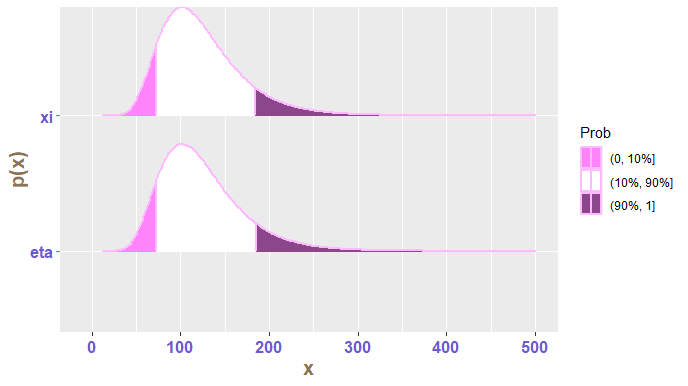
\includegraphics[width=0.95\linewidth]{img/plot12_n2_new.png}
					\caption{$\sigma_{1} = 0.5$, $\sigma_{2} = 0.5$. } %% подпись к рисунку
					\label{ris7} %% метка рисунка для ссылки на него
				\end{minipage}
				
			\end{center}
		\end{figure}
		
		\note{Построим оценки плотности для $\xi$ и $\eta$, когда ошибки имеют очень маленькие значения и когда достаточно большие. На данном графике представлен случай $\sigma_{1}^{2} = 0.25$, $\sigma_{2}^{2} = 0.25$, при этом ошибки $q_{10}$, $q_{50}$, $q_{90}$ близки к нулю.}
		
	\end{frame}
	
	\begin{frame}{Часть 4: Точность аппроксимации}
		
		Теперь посмотрим на случай, когда ошибки аппроксимации достаточно большие. Получили $err_{med} = 20.9\%$,  $err_{q_{10}} = 66.7\%$,  $err_{q_{90}} = 19.1\%$.
		
		\begin{figure}[h]
			\begin{center}
				\begin{minipage}[h]{1\linewidth}
					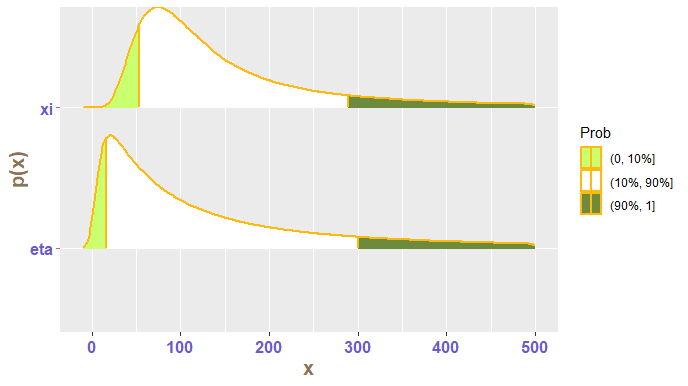
\includegraphics[width=0.95\linewidth]{img/plot12_n1_new.png}
					\caption{$\sigma_{1} = 1.5$, $\sigma_{2} = 0.5$. } %% подпись к рисунку
					\label{ris7} %% метка рисунка для ссылки на него
				\end{minipage}
				
			\end{center}
		\end{figure}
	
	\note{Построим оценки плотности для $\xi$ и $\eta$, когда ошибки имеют очень маленькие значения и когда достаточно большие. На данном графике представлен случай $\sigma_{1}^{2} = 0.25$, $\sigma_{2}^{2} = 0.25$, при этом ошибки $q_{10}$, $q_{50}$, $q_{90}$ близки к нулю.}
		
	\end{frame}
	
	\begin{frame}{Заключение}

		\textcolor{blue}{\hbox{\textbf{Мною были получены следующие результаты:}}}
		\begin{enumerate}
			\item Получено условие на $\sigma$ для существования трехточечной симметричной вероятностной аппроксимации логнормального распределения.
			\item Численно оценена точность аппроксимации математического ожидания и дисперсии логнормального распределения с помощью метода Свонсона, применяемого к нормальному распределению.
			\item Формально и полно написано обоснование алгоритма для нахождения трехточечной симметричной аппроксимации произведения логнормальных распределений.
			\item Построен алгоритм для нахождения трехточечной симметричной аппроксимации суммы логнормальных распределений.
			\item Численно оценена точность трехточечной симметричной аппроксимации суммы логнормальных распределений.
		\end{enumerate}
		%\bigskip
		
		\note{Таким образом, мною были получены следующие результаты. 
			Получено условие на $\sigma$ для существования трехточечной симметричной аппроксимации логнормального распределения.
			Численно оценена точность аппроксимации мат. ожидания и дисперсии логнормального распределения с помощью метода Свонсона, применяемого к нормальному распределению.
			Построен алгоритм для нахождения трехточечной симметричной аппроксимации суммы логнормальных распределений.
			Численно оценена точность трехточечной аппроксимации суммы логнормальных распределений.}
		
	\end{frame}

	
\end{document}